\chapter{Diseño y arquitectura del sistema}
\label{capitulo3}
\lhead{Capítulo 3. \emph{Diseño del sistema}}

En este capitulo se explicará la arquitectura, el diseño y el modo en el que el IDS basado en SSM interactuara con Bro. Además, se detallaran las salidas y los datos de configuración que va a considerar el sistema para su correcto funcionamiento vas a considerar. Este capitulo tiene la intención de mostrar la visión general del modelado del sistema que se realizo a partir de las bases teóricas.

\section{Arquitectura del sistema}

La arquitectura del detector de intrusiones que se muestra en el presente trabajo se basa en una arquitectura modular la cual está conformada por tres modulo. Un modulo para realizar la segmentación de los URIs, otro  para realizar la evaluación y un tercero para realizar el entrenamiento y de esta forma crear un modelo de normalidad.

A grandes rasgos, el modulo de segmentación se encargará de tomar el URI que proviene de la solicitud de tipo GET o HEAD que se le hace al servidor HTTP, normalizarlo y segmentarlo siguiendo las especificaciones del RFC (insertar nombre del RFC) .

Por otra parte, el modulo de evaluación se encargará de evaluar la probabilidad de generación de cada uno de los segmentos del URI generados por el modulo de segmentación para al final decidir si el URI de la solicitud enviada al servidor de tipo HTTP es anómalo o no.

Por último, el modulo de entrenamiento será el encargado de crear el modelo de normalidad del sistema. Para esto, el sistema recibirá solicitudes libres de ataques e irá calculando la probabilidad de aparición de cada una de las palabras que aparecen en las mismas.

Tanto el modulo de evaluación, como el modulo de entrenamiento son dependientes del modulo de segmentación ya que requieren de los segmentos de URI generados por eso para realizar su trabajo. 

La arquitectura del sistema queda detallada en la figura \ref{fig:arquitectura}.

\begin{figure}[tb]
\begin{center}
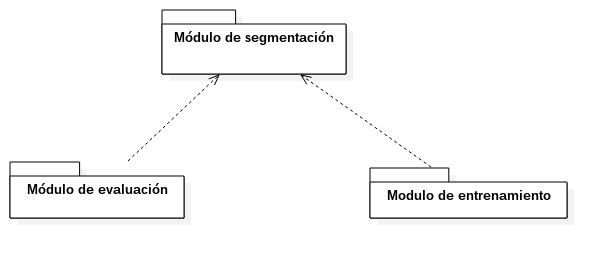
\includegraphics[width=3in]{arquitectura.png}
\caption{Arquitectura del sistema.}
\label{fig:arquitectura}
\end{center}
\end{figure}

\begin{itemize}
\item Modo evaluación: En este modo de operación solo se activaran los módulos de segmentación y evaluación del sistema. A manera general, esta modalidad, se encargará de recibir peticiones de tipo HTTP/GET, extraer su URI y segmentarlos a tráves del modulo de segmentación para luego evaluar si  el mismo es anómalo o no, haciendo uso del modulo de evaluación. El funcionamiento de esta modalidad queda detallado en la figura \ref{fig:modoSistema}.
\item Modo entrenamiento ``Online'': En este modo de operación solo trabajaran los módulos de segmentación y entrenamiento. Esta modalidad es un tipo de entrenamiento en donde se toman peticiones de tipo HTTP/GET y se segmenta el URI que se encuentran en las mismas haciendo uso del modulo de segmentación. Una vez realizado esto, el modulo de entrenamiento tomara los segmentos arrojados por el modulo de segmentación, calculara la probabilidad de aparición de los mismos para de esta manera ir modificando un modelo de normalidad previamente establecido, es decir, la salida de este modo de entrenamiento sera la de el modelo previamente establecido con ciertas modificaciones realizadas a partir de las observaciones hechas. El funcionamiento de esta modalidad queda detallado en la figura \ref{fig:modoSistema}..
\item Modo entrenamiento ``Offline'': Esta modalidad del sistema en análoga al modo de entrenamiento ``Online''. El único aspecto que diferencia a ambas modalidades es que cuando el sistema funciona en modo ``Offline'' no se toma en cuenta, ni se modifica un modelo de normalidad previamente construido. La salida de este modo de entrenamiento sera un modelo de normalidad construido desde cero.El funcionamiento de esta modalidad queda detallado en la figura \ref{fig:modoSistema}.
\end{itemize}

\begin{figure}[tb]
\begin{center}
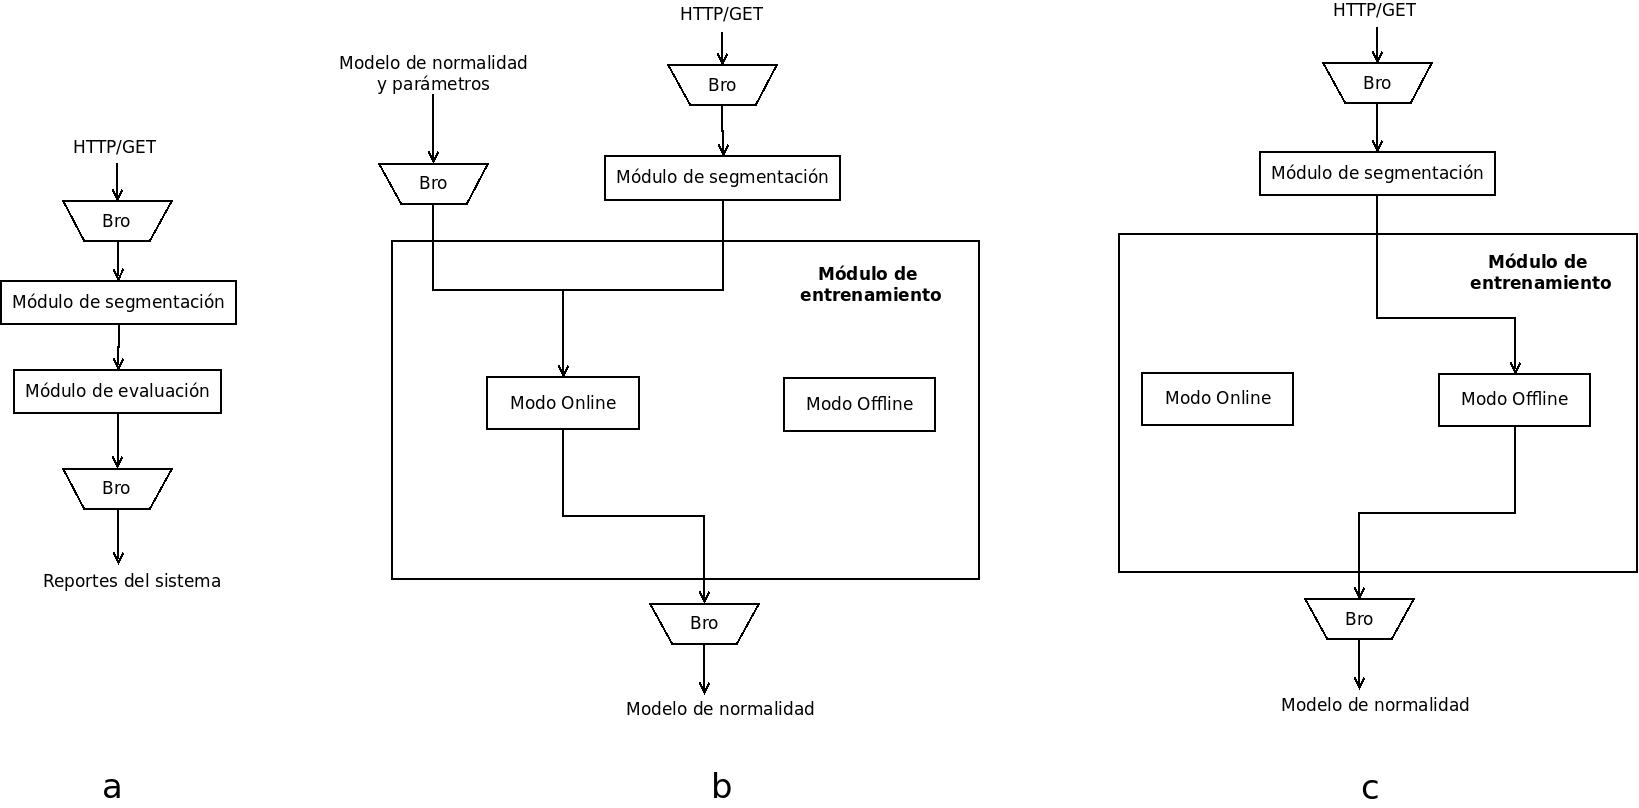
\includegraphics[width=\linewidth]{modoOperacion.jpeg}
\caption{Modo evaluación (a), modo entrenamiento ``Online'' (b), modo entrenamiento ``Offline'' (c).}
\label{fig:modoSistema}
\end{center}
\end{figure}

\section{Módulos}

En esta sección se describirán las tareas de cada uno de los módulos que conformar la arquitectura detallada en la figura \ref{fig:arquitectura}, el modo en el que se subdividieron dichas tareas, los datos de entrada y salida, y la interacción que existe entre los mismos.

\subsection{Modulo de segmentación}

El modulo de segmentación es un elemento clave dentro de la construcción del IDS basado en SSM, es por eso que su buen diseño e implementación es importante para el buen funcionamiento del sistema. Este se encarga, como se menciono anteriormente,de tomar el URI que proviene de la solicitud de tipo GET o HEAD que se le hace al servidor HTTP capturado por Bro, normalizarlo y segmentarlo siguiendo las especificaciones del RFC (insertar nombre del RFC) 

Es evidente entonces, que este modulo consta de dos funcionalidades fundamentales: la normalización de los URIs y la segmentación.  La normalización se encargará de tomar el URI de las peticiones HTTP entrantes y codificarlo a formato UTF-8. Normalizar es un paso importante dentro del sistema  ya que se estandarizar la forma en las que están escritos los URIs facilita tanto la evaluación como el entrenamiento en el sistema. Por otra parte, el output arrojado por esta función de normalización será tomado por la de segmentación, quien a su vez se encargará de segmentar el URI de la forma en la que se explica en la sección \ref{sec:delimitadores}, es decir, el URI se dividirá en las diferentes partes estipuladas en el RFC 3986: el ``host'', la ruta, los argumentos, los valores y el ``fragment''.

 En las base teórica, la segmentación de los URIs se realiza mediante un autómata que se encarga de reconocer (realizar un análisis sintáctico) y evaluar en cada uno de sus estados la probabilidad de generación de cada uno de los segmentos.  No obstante, en la función de segmentación del sistema implementado, esta tarea se modeló mediante un analizador sintáctico que hace uso de una gramática (libre de contexto) de atributos que genera el mismo lenguaje que reconoce el autómata presentado en la figura ~\ref{fig:automata}, es decir, el lenguaje de los URI.

En la figura (insertar nombre de la figura) se puede apreciar el diagrama de bloques que refleja el funcionamiento del módulo de segmentación.

\begin{figure}[tb]
\begin{center}
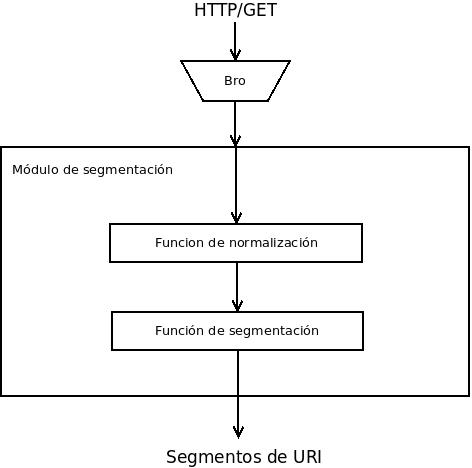
\includegraphics[width=3in]{segArquiCompleta.jpeg}
\caption{Diagrama de bloques del módulo de segmentación.}
\label{fig:modoSistema}
\end{center}
\end{figure}

*************************************************************************8
Dentro de este modulo se pueden contemplar dos grandes funcionalidades: la normalización y la segmentación.

En la normalización se encargará de traducir los URIs entrantes al formato UTF-8, mientras que, la segmentación tendrá el trabajo de dividir los URIs en segmentos. 

``En el capítulo 3, se pudo apreciar la arquitectura del módulo de segmentación. Además, se pudo observar que el mismo consta de dos funcionalidades fundamentales: la normalización de los URIs y la segmentación. A grandes rasgos, la normalización se encargará de tomar el URI de las peticiones HTTP entrantes y codificarlo a formato UTF-8, el output arrojado por esta función será tomado por la de segmentación, quien a su vez se encargará de segmentar el URI de la forma en la que se explica en la sección \ref{sec:delimitadores}, es decir, el URI se dividirá en las diferentes partes estipuladas en el RFC 3986: el host, el path, los argumentos, los valores y el fragment''

``El problema a resolver, presenta dos tareas fundamentales: segmentar y realizar un análisis sintáctico. En programación cuando se tiene un conjunto de datos de entrada (en este caso serían los URIs), y se desea realizar un análisis sintáctico sobre el mismo, lo más común es implementar un analizador sintáctico o parser.

El análisis realizado por un analizador sintáctico “es el proceso en el cual se estudia la manera en la que una cadena de caracteres terminales es generado por una gramática.”  Compiler, principle, techniques and tools."

Por otra parte, existen varios tipos de gramáticas, las gramáticas libre de contexto y las gramáticas regulares. Las que se suelen utilizar en un analizador sintáctico son las gramáticas libres de contexto. Una gramática libre de contexto “en el contexto del lenguaje natural, sería un conjunto de reglas que son utilizadas para construir o validar oraciones” “Formal Languages and Automata Theory” de D. Goswami and K. V. Krishna. 

De manera más formal, según la definición 3.1.1 de: “Formal Languages and Automata Theory” de D. Goswami and K. V. Krishna. Se puede decir que una gramática libre de contexto es una  cuádrupla G = (N, $\sum$, P, S), donde:
\begin{enumerate}
\item N es un conjunto de no-terminales,
\item $\sum$ es un conjunto de terminales. Los terminales son elementos fundamentales en el lenguaje generado por la gramática.
\item S $\in$ N es el símbolo de inicio.
\item P es un subconjunto finito de N x V * llamado el conjunto de reglas de producciones. Aquí, V = N U $\sum$."
\end{enumerate}

Entonces, para realizar el analizador sintáctico se requiere construir una gramática libre de contexto que genere el mismo lenguaje que reconoce el autómata presentado en la imagen ~\ref{fig:automata}, es decir, el lenguaje de los URI.

Antes de presentar la gramática se mostrarán los tokens que utilizará la misma como elementos terminales. Un token “es la cadena de caracteres más corta que posee algún significado” Scott, Compilers.''




A continuación se explicará con mas detalle ambas funcionalidades. 

``La normalización es un paso importante dentro del modulo de segmentación ya que se encarga de estandarizar la forma en las que están escritos los URIs para de este modo facilitar tanto la evaluación como el entrenamiento en el sistema.''

\subsection{Modulo de evaluación}
\label{sec:evaluacion}

Este modulo, como se mencionó con anterioridad es el encargado de evaluar la probabilidad de generación de cada uno de los segmentos del URI dado un modelo de normalidad. Una vez calculadas estas probabilidades, el modulo se encargará de calcular un índice de anormalidad del URI mediante el uso de las formulas descritas en la sección ~\ref{subsec:exprIndice} para luego compararlo con un parámetro $\theta$ y de este modo saber si el URI posee alguna anormalidad o no. 


\subsection{Modulo de entrenamiento}\label{sec:entrenamiento}

El modelo de normalidad es uno de los aspecto importantes dentro del IDS basado en SSM ya que a partir de la información que este almacena se podrá decidir si un URI es anómalo o no dependiendo de la similitud que posea este con los datos que almacena el modelo. Por esta razón, realizar un modelo de normalidad apropiado es un aspecto  importante para que el módulo de evaluación haga detecciones de intrusiones más certeras.

El módulo encargado de elaborar los modelos de normalidad será el módulo de entrenamiento. A grandes rasgos, este se encargará de recibir solicitudes libres de ataques e irá calculando la probabilidad de aparición de cada una de las palabras que aparecen en los URIs de las mismas, para finalmente dar al sistema una lista de palabras observadas junto con su probabilidad de aparición.

En esta sección se explicará con detalles el funcionamiento y las expresiones utilizadas por el módulo de entrenamiento para construir el modelo de normalidad del sistema. 

``Este módulo de entrenamiento será el encargado de armar el vocabulario del módulo de normalidad del sistema. Como se mencionó con anterioridad, este módulo tomará un conjunto de solicitudes libres de ataques, para luego calcular la probabilidad de aparición de las palabras en el conjunto de observaciones totales de cada uno de los estados. En términos más formales, la  tarea que realiza este módulo se puede modelar de la siguiente forma:''